% Options for packages loaded elsewhere
\PassOptionsToPackage{unicode}{hyperref}
\PassOptionsToPackage{hyphens}{url}
\PassOptionsToPackage{dvipsnames,svgnames,x11names}{xcolor}
%
\documentclass[
  letterpaper,
  DIV=11,
  numbers=noendperiod,
  oneside]{scrartcl}

\usepackage{amsmath,amssymb}
\usepackage{iftex}
\ifPDFTeX
  \usepackage[T1]{fontenc}
  \usepackage[utf8]{inputenc}
  \usepackage{textcomp} % provide euro and other symbols
\else % if luatex or xetex
  \usepackage{unicode-math}
  \defaultfontfeatures{Scale=MatchLowercase}
  \defaultfontfeatures[\rmfamily]{Ligatures=TeX,Scale=1}
\fi
\usepackage{lmodern}
\ifPDFTeX\else  
    % xetex/luatex font selection
\fi
% Use upquote if available, for straight quotes in verbatim environments
\IfFileExists{upquote.sty}{\usepackage{upquote}}{}
\IfFileExists{microtype.sty}{% use microtype if available
  \usepackage[]{microtype}
  \UseMicrotypeSet[protrusion]{basicmath} % disable protrusion for tt fonts
}{}
\makeatletter
\@ifundefined{KOMAClassName}{% if non-KOMA class
  \IfFileExists{parskip.sty}{%
    \usepackage{parskip}
  }{% else
    \setlength{\parindent}{0pt}
    \setlength{\parskip}{6pt plus 2pt minus 1pt}}
}{% if KOMA class
  \KOMAoptions{parskip=half}}
\makeatother
\usepackage{xcolor}
\usepackage[left=1in,marginparwidth=2.0666666666667in,textwidth=4.1333333333333in,marginparsep=0.3in]{geometry}
\setlength{\emergencystretch}{3em} % prevent overfull lines
\setcounter{secnumdepth}{-\maxdimen} % remove section numbering
% Make \paragraph and \subparagraph free-standing
\ifx\paragraph\undefined\else
  \let\oldparagraph\paragraph
  \renewcommand{\paragraph}[1]{\oldparagraph{#1}\mbox{}}
\fi
\ifx\subparagraph\undefined\else
  \let\oldsubparagraph\subparagraph
  \renewcommand{\subparagraph}[1]{\oldsubparagraph{#1}\mbox{}}
\fi

\usepackage{color}
\usepackage{fancyvrb}
\newcommand{\VerbBar}{|}
\newcommand{\VERB}{\Verb[commandchars=\\\{\}]}
\DefineVerbatimEnvironment{Highlighting}{Verbatim}{commandchars=\\\{\}}
% Add ',fontsize=\small' for more characters per line
\usepackage{framed}
\definecolor{shadecolor}{RGB}{241,243,245}
\newenvironment{Shaded}{\begin{snugshade}}{\end{snugshade}}
\newcommand{\AlertTok}[1]{\textcolor[rgb]{0.68,0.00,0.00}{#1}}
\newcommand{\AnnotationTok}[1]{\textcolor[rgb]{0.37,0.37,0.37}{#1}}
\newcommand{\AttributeTok}[1]{\textcolor[rgb]{0.40,0.45,0.13}{#1}}
\newcommand{\BaseNTok}[1]{\textcolor[rgb]{0.68,0.00,0.00}{#1}}
\newcommand{\BuiltInTok}[1]{\textcolor[rgb]{0.00,0.23,0.31}{#1}}
\newcommand{\CharTok}[1]{\textcolor[rgb]{0.13,0.47,0.30}{#1}}
\newcommand{\CommentTok}[1]{\textcolor[rgb]{0.37,0.37,0.37}{#1}}
\newcommand{\CommentVarTok}[1]{\textcolor[rgb]{0.37,0.37,0.37}{\textit{#1}}}
\newcommand{\ConstantTok}[1]{\textcolor[rgb]{0.56,0.35,0.01}{#1}}
\newcommand{\ControlFlowTok}[1]{\textcolor[rgb]{0.00,0.23,0.31}{#1}}
\newcommand{\DataTypeTok}[1]{\textcolor[rgb]{0.68,0.00,0.00}{#1}}
\newcommand{\DecValTok}[1]{\textcolor[rgb]{0.68,0.00,0.00}{#1}}
\newcommand{\DocumentationTok}[1]{\textcolor[rgb]{0.37,0.37,0.37}{\textit{#1}}}
\newcommand{\ErrorTok}[1]{\textcolor[rgb]{0.68,0.00,0.00}{#1}}
\newcommand{\ExtensionTok}[1]{\textcolor[rgb]{0.00,0.23,0.31}{#1}}
\newcommand{\FloatTok}[1]{\textcolor[rgb]{0.68,0.00,0.00}{#1}}
\newcommand{\FunctionTok}[1]{\textcolor[rgb]{0.28,0.35,0.67}{#1}}
\newcommand{\ImportTok}[1]{\textcolor[rgb]{0.00,0.46,0.62}{#1}}
\newcommand{\InformationTok}[1]{\textcolor[rgb]{0.37,0.37,0.37}{#1}}
\newcommand{\KeywordTok}[1]{\textcolor[rgb]{0.00,0.23,0.31}{#1}}
\newcommand{\NormalTok}[1]{\textcolor[rgb]{0.00,0.23,0.31}{#1}}
\newcommand{\OperatorTok}[1]{\textcolor[rgb]{0.37,0.37,0.37}{#1}}
\newcommand{\OtherTok}[1]{\textcolor[rgb]{0.00,0.23,0.31}{#1}}
\newcommand{\PreprocessorTok}[1]{\textcolor[rgb]{0.68,0.00,0.00}{#1}}
\newcommand{\RegionMarkerTok}[1]{\textcolor[rgb]{0.00,0.23,0.31}{#1}}
\newcommand{\SpecialCharTok}[1]{\textcolor[rgb]{0.37,0.37,0.37}{#1}}
\newcommand{\SpecialStringTok}[1]{\textcolor[rgb]{0.13,0.47,0.30}{#1}}
\newcommand{\StringTok}[1]{\textcolor[rgb]{0.13,0.47,0.30}{#1}}
\newcommand{\VariableTok}[1]{\textcolor[rgb]{0.07,0.07,0.07}{#1}}
\newcommand{\VerbatimStringTok}[1]{\textcolor[rgb]{0.13,0.47,0.30}{#1}}
\newcommand{\WarningTok}[1]{\textcolor[rgb]{0.37,0.37,0.37}{\textit{#1}}}

\providecommand{\tightlist}{%
  \setlength{\itemsep}{0pt}\setlength{\parskip}{0pt}}\usepackage{longtable,booktabs,array}
\usepackage{calc} % for calculating minipage widths
% Correct order of tables after \paragraph or \subparagraph
\usepackage{etoolbox}
\makeatletter
\patchcmd\longtable{\par}{\if@noskipsec\mbox{}\fi\par}{}{}
\makeatother
% Allow footnotes in longtable head/foot
\IfFileExists{footnotehyper.sty}{\usepackage{footnotehyper}}{\usepackage{footnote}}
\makesavenoteenv{longtable}
\usepackage{graphicx}
\makeatletter
\def\maxwidth{\ifdim\Gin@nat@width>\linewidth\linewidth\else\Gin@nat@width\fi}
\def\maxheight{\ifdim\Gin@nat@height>\textheight\textheight\else\Gin@nat@height\fi}
\makeatother
% Scale images if necessary, so that they will not overflow the page
% margins by default, and it is still possible to overwrite the defaults
% using explicit options in \includegraphics[width, height, ...]{}
\setkeys{Gin}{width=\maxwidth,height=\maxheight,keepaspectratio}
% Set default figure placement to htbp
\makeatletter
\def\fps@figure{htbp}
\makeatother
\newlength{\cslhangindent}
\setlength{\cslhangindent}{1.5em}
\newlength{\csllabelwidth}
\setlength{\csllabelwidth}{3em}
\newlength{\cslentryspacingunit} % times entry-spacing
\setlength{\cslentryspacingunit}{\parskip}
\newenvironment{CSLReferences}[2] % #1 hanging-ident, #2 entry spacing
 {% don't indent paragraphs
  \setlength{\parindent}{0pt}
  % turn on hanging indent if param 1 is 1
  \ifodd #1
  \let\oldpar\par
  \def\par{\hangindent=\cslhangindent\oldpar}
  \fi
  % set entry spacing
  \setlength{\parskip}{#2\cslentryspacingunit}
 }%
 {}
\usepackage{calc}
\newcommand{\CSLBlock}[1]{#1\hfill\break}
\newcommand{\CSLLeftMargin}[1]{\parbox[t]{\csllabelwidth}{#1}}
\newcommand{\CSLRightInline}[1]{\parbox[t]{\linewidth - \csllabelwidth}{#1}\break}
\newcommand{\CSLIndent}[1]{\hspace{\cslhangindent}#1}

\usepackage{booktabs}
\usepackage{longtable}
\usepackage{array}
\usepackage{multirow}
\usepackage{wrapfig}
\usepackage{float}
\usepackage{colortbl}
\usepackage{pdflscape}
\usepackage{tabu}
\usepackage{threeparttable}
\usepackage{threeparttablex}
\usepackage[normalem]{ulem}
\usepackage{makecell}
\usepackage{xcolor}
\KOMAoption{captions}{tableheading}
\makeatletter
\makeatother
\makeatletter
\makeatother
\makeatletter
\@ifpackageloaded{caption}{}{\usepackage{caption}}
\AtBeginDocument{%
\ifdefined\contentsname
  \renewcommand*\contentsname{Table of contents}
\else
  \newcommand\contentsname{Table of contents}
\fi
\ifdefined\listfigurename
  \renewcommand*\listfigurename{List of Figures}
\else
  \newcommand\listfigurename{List of Figures}
\fi
\ifdefined\listtablename
  \renewcommand*\listtablename{List of Tables}
\else
  \newcommand\listtablename{List of Tables}
\fi
\ifdefined\figurename
  \renewcommand*\figurename{Figure}
\else
  \newcommand\figurename{Figure}
\fi
\ifdefined\tablename
  \renewcommand*\tablename{Table}
\else
  \newcommand\tablename{Table}
\fi
}
\@ifpackageloaded{float}{}{\usepackage{float}}
\floatstyle{ruled}
\@ifundefined{c@chapter}{\newfloat{codelisting}{h}{lop}}{\newfloat{codelisting}{h}{lop}[chapter]}
\floatname{codelisting}{Listing}
\newcommand*\listoflistings{\listof{codelisting}{List of Listings}}
\makeatother
\makeatletter
\@ifpackageloaded{caption}{}{\usepackage{caption}}
\@ifpackageloaded{subcaption}{}{\usepackage{subcaption}}
\makeatother
\makeatletter
\@ifpackageloaded{tcolorbox}{}{\usepackage[skins,breakable]{tcolorbox}}
\makeatother
\makeatletter
\@ifundefined{shadecolor}{\definecolor{shadecolor}{rgb}{.97, .97, .97}}
\makeatother
\makeatletter
\makeatother
\makeatletter
\@ifpackageloaded{sidenotes}{}{\usepackage{sidenotes}}
\@ifpackageloaded{marginnote}{}{\usepackage{marginnote}}
\makeatother
\makeatletter
\makeatother
\ifLuaTeX
  \usepackage{selnolig}  % disable illegal ligatures
\fi
\IfFileExists{bookmark.sty}{\usepackage{bookmark}}{\usepackage{hyperref}}
\IfFileExists{xurl.sty}{\usepackage{xurl}}{} % add URL line breaks if available
\urlstyle{same} % disable monospaced font for URLs
\hypersetup{
  pdftitle={Report on the use of passive acoustic monitoring for evaluating ecological integrity in Prince Edward Island National Park},
  pdfauthor={Alex MacPhail},
  colorlinks=true,
  linkcolor={blue},
  filecolor={Maroon},
  citecolor={Blue},
  urlcolor={Blue},
  pdfcreator={LaTeX via pandoc}}

\title{Report on the use of passive acoustic monitoring for evaluating
ecological integrity in Prince Edward Island National Park}
\author{Alex MacPhail}
\date{2024-01-31}

\begin{document}
\maketitle
\ifdefined\Shaded\renewenvironment{Shaded}{\begin{tcolorbox}[boxrule=0pt, borderline west={3pt}{0pt}{shadecolor}, sharp corners, frame hidden, breakable, enhanced, interior hidden]}{\end{tcolorbox}}\fi

\renewcommand*\contentsname{Table of contents}
{
\hypersetup{linkcolor=}
\setcounter{tocdepth}{3}
\tableofcontents
}
\begin{Shaded}
\begin{Highlighting}[]
\DocumentationTok{\#\#\# To run this locally}

\CommentTok{\# Open RStudio or your preferred IDE}
\CommentTok{\# Create a new project and set up for version control using the GitHub repository}
\CommentTok{\# Pull from remote main}
\CommentTok{\# Load the pei.RData file}
\CommentTok{\# Render the document and review the results}
\end{Highlighting}
\end{Shaded}

\begin{figure}

{\centering 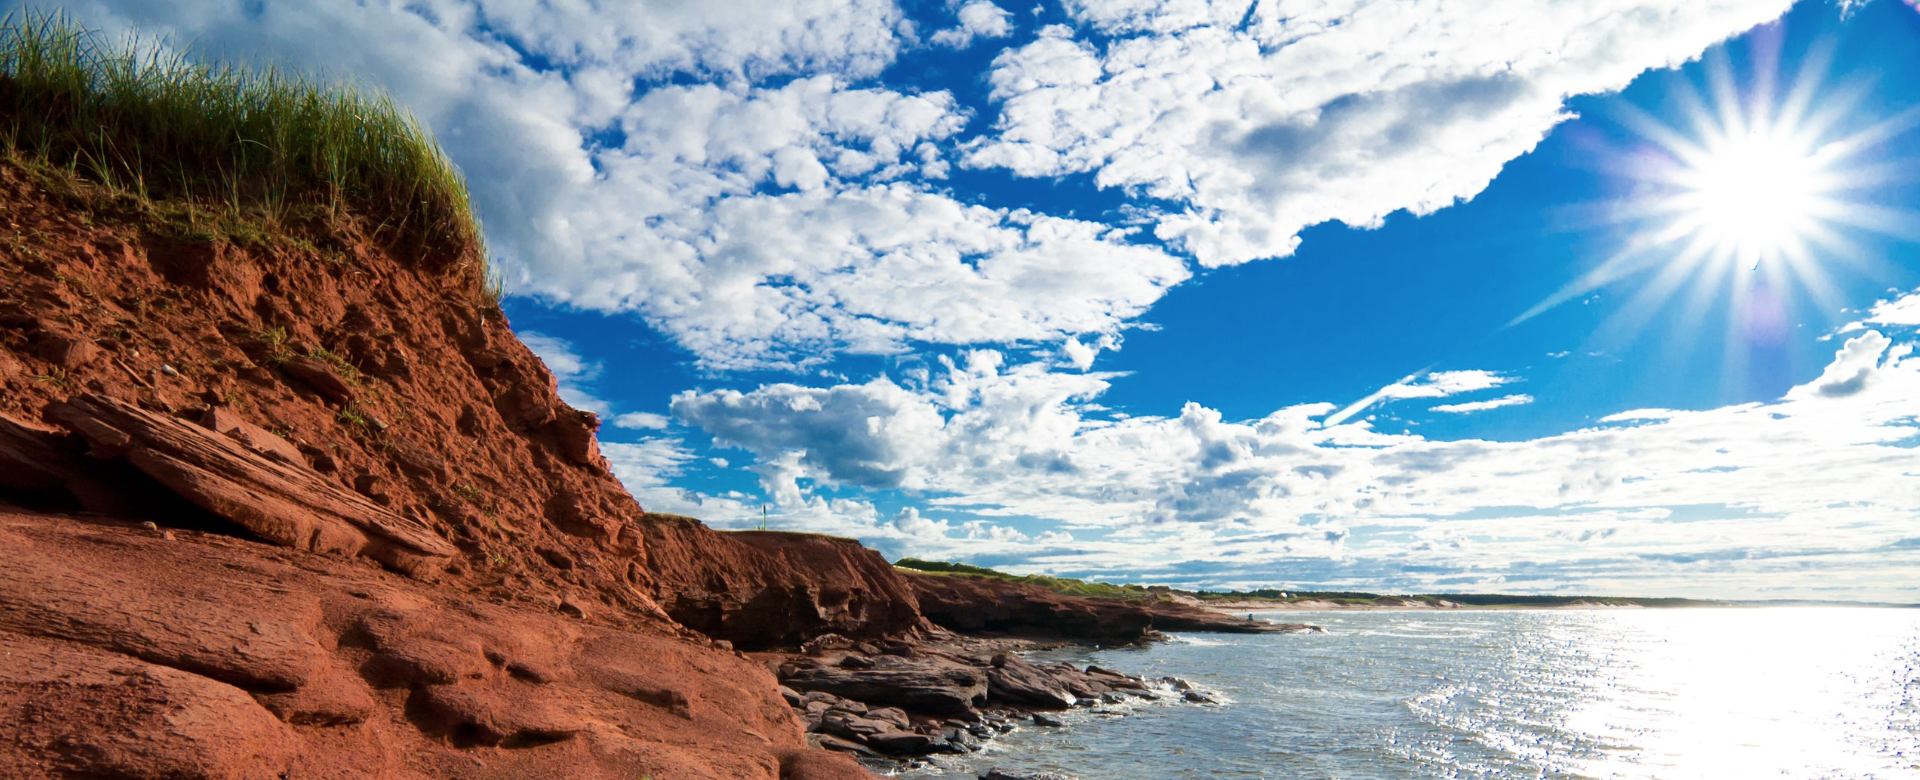
\includegraphics{peinpheader.png}

}

\end{figure}

\hypertarget{abstract}{%
\section{Abstract}\label{abstract}}

\begin{center}\rule{0.5\linewidth}{0.5pt}\end{center}

\hypertarget{introduction}{%
\section{Introduction}\label{introduction}}

Human activities have been identified as key contributors to the global
decline in forest wildlife. The repercussions of habitat fragmentation
and loss, climate change, and increased access to sensitive areas exert
direct and indirect pressures on forest biodiversity, particularly in
managed regions.

In 2019, Prince Edward Island National Park initiated a program
incorporating autonomous recording units (ARUs) for passive acoustic
monitoring (PAM) of the Park's wildlife. ARUs are compact environmental
sensors that are designed to passively record the environment, capturing
vocalizing species like birds and amphibians. This technology enables
resource managers to conduct prolonged surveys with minimal human
interference. The species detected by these units contribute valuable
information to ecological integrity metrics such as species richness,
diversity, occupancy, and trends over time. This data aids
decision-making and management within the Park. Given the rapid and ease
of accumulating data from these units, maintaining a high standard of
data integrity is paramount to ensure future data interoperability and
sharing. WildTrax, an online platform tailored for users of
environmental sensors, addresses this challenge by providing a solution
to standardize, harmonize, and share data.

The objectives of this report are to:

\begin{itemize}
\tightlist
\item
  Describe the data management and processing procedures for the
  acoustic data collected from 2019 to 2023
\item
  Identify all audible species and quantify the abundance of each
  species within each recording
\item
  Define straightforward methods and robust ecological integrity metrics
  for evaluating species presence, species richness, and species
  occupancy over time at various locations
\item
  Offer recommendations for ongoing monitoring approaches to contribute
  to the assessment of ecological integrity in forest ecosystems
\item
  Facilitate data publication to the public, resource managers, academic
  institutions, and other relevant agencies
\end{itemize}

\begin{center}\rule{0.5\linewidth}{0.5pt}\end{center}

\hypertarget{methods}{%
\section{Methods}\label{methods}}

\hypertarget{data-collection}{%
\subsection{Data collection}\label{data-collection}}

Data were collected during the spring and summer seasons from 2019 to
2023. A total of 30 locations were surveyed over the five-year period:

\begin{itemize}
\tightlist
\item
  21 locations as part of the forest songbird monitoring program (code:
  \texttt{PENP-*}) with ARUs recording during the morning hours,
\item
  6 for Bank Swallow Monitoring (code: \texttt{PENP-BS-*}) with ARUs
  placed strategically beside ponds recording in the evening,
\item
  2 locations deployed in First Nations communities
  (\texttt{ASC-1,\ LXI-1}) to complement the forest songbird and evening
  schedules,
\item
  And one location for events (\texttt{PENP-E1}), which was to examine
  the effects of a single public event
\end{itemize}

Nine locations (PENP-1-1, PENP-1-2, PENP-2-3, PENP-3-1, PENP-3-2,
PENP-4-1, PENP-4-2, PENP-4-3, PENP-4-4) were surveyed each year, while
the remaining locations were surveyed on rotation as best as possible.
Details can be found in Table 1 (Table~\ref{tbl-loc-summary}) and
illustrated in Figure 1 (Figure~\ref{fig-locs}). ARUs were deployed at
the beginning of the breeding season in April and May. These ARUs
rotated through locations during the spring and summer until their final
retrieval in July and August. At each location, the ARUs were set to
record for 30 minutes continuously every hour for four hours, starting
one hour before dawn and ending three hours after dawn. For Bank Swallow
Monitoring locations, recordings were made every 5 minutes for a
duration of 3 minutes each from 1.5 hours before dusk to 1.5 hours after
dusk. On average, each ARU recorded for 11.27 +/- 8.03 days.

\begin{figure}

{\centering 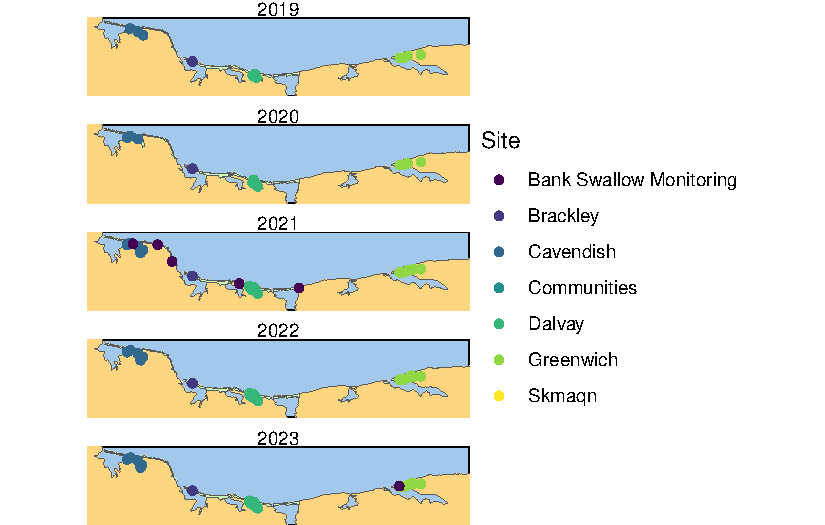
\includegraphics{peinp_files/figure-pdf/fig-locs-1.pdf}

}

\caption{\label{fig-locs}Locations surveyed each year}

\end{figure}

\hypertarget{tbl-loc-summary}{}
\begin{margintable}

\begin{table}

\caption{\label{tbl-loc-summary}Locations surveyed across years. Ones indicated a deployment in that
year for that location }Location summary for ARUs deployed}
\centering
\begin{tabular}[t]{l|r|r|r|r|r|l}
\hline
Location & 2019 & 2020 & 2021 & 2022 & 2023 & Site\\
\hline
PENP-1-1 & 1 & 1 & 1 & 1 & 1 & Cavendish\\
\hline
PENP-1-2 & 1 & 1 & 1 & 1 & 1 & Cavendish\\
\hline
PENP-1-3 & 1 & 0 & 1 & 1 & 0 & Cavendish\\
\hline
PENP-2-3 & 1 & 1 & 1 & 1 & 1 & Brackley\\
\hline
PENP-3-1 & 1 & 1 & 1 & 1 & 1 & Dalvay\\
\hline
PENP-3-2 & 1 & 1 & 1 & 1 & 1 & Dalvay\\
\hline
PENP-3-4 & 1 & 0 & 1 & 1 & 1 & Dalvay\\
\hline
PENP-4-1 & 1 & 1 & 1 & 1 & 1 & Greenwich\\
\hline
PENP-4-2 & 1 & 1 & 1 & 1 & 1 & Greenwich\\
\hline
PENP-4-3 & 1 & 1 & 1 & 1 & 1 & Greenwich\\
\hline
PENP-4-4 & 1 & 1 & 1 & 1 & 1 & Greenwich\\
\hline
PENP-1-4 & 0 & 1 & 1 & 1 & 1 & Cavendish\\
\hline
PENP-3-5 & 0 & 1 & 1 & 1 & 1 & Dalvay\\
\hline
PENP-3-6 & 0 & 1 & 1 & 1 & 1 & Dalvay\\
\hline
ASC-1 & 0 & 0 & 1 & 0 & 0 & Communities\\
\hline
LXI-1 & 0 & 0 & 1 & 0 & 0 & Communities\\
\hline
PENP-1-5 & 0 & 0 & 1 & 1 & 1 & Cavendish\\
\hline
PENP-1-6 & 0 & 0 & 1 & 1 & 1 & Cavendish\\
\hline
PENP-3-7 & 0 & 0 & 1 & 1 & 1 & Dalvay\\
\hline
PENP-3-8 & 0 & 0 & 1 & 1 & 1 & Dalvay\\
\hline
PENP-4-6 & 0 & 0 & 1 & 1 & 1 & Greenwich\\
\hline
PENP-5-1 & 0 & 0 & 1 & 1 & 1 & Skmaqn\\
\hline
PENP-BS-1 & 0 & 0 & 1 & 0 & 0 & Bank Swallow Monitoring\\
\hline
PENP-BS-2 & 0 & 0 & 1 & 0 & 0 & Bank Swallow Monitoring\\
\hline
PENP-BS-3 & 0 & 0 & 1 & 0 & 0 & Bank Swallow Monitoring\\
\hline
PENP-BS-4 & 0 & 0 & 1 & 0 & 0 & Bank Swallow Monitoring\\
\hline
PENP-BS-5 & 0 & 0 & 1 & 0 & 0 & Bank Swallow Monitoring\\
\hline
PENP-4-5 & 0 & 0 & 0 & 1 & 1 & Greenwich\\
\hline
PENP-E1 & 0 & 0 & 0 & 1 & 0 & Skmaqn\\
\hline
PENP-BS-6 & 0 & 0 & 0 & 0 & 1 & Bank Swallow Monitoring\\
\hline
\end{tabular}
\end{table}

\end{margintable}

\hypertarget{data-management}{%
\subsection{Data management}\label{data-management}}

A total of 10078 recordings were collected (see
Figure~\ref{fig-recs-collect}). From 2019 - 2021, data were transferred
via hard drive to the University of Alberta in Edmonton, where they are
redundantly stored on a server known as Cirrus. The recordings were
standardized to ensure adherence to the naming convention of
\texttt{LOCATION\_DATETIME}, such as
\texttt{PENP-1-1\_20230625\_053500.wav}. The remaining recordings (2022
- 2023) were directly uploaded to WildTrax by Parks Canada staff and can
be downloaded from the platform's Recording tab, accessible under Manage
\textgreater{} Download list of recordings (see
Figure~\ref{fig-download-recs}).

\begin{figure}

{\centering 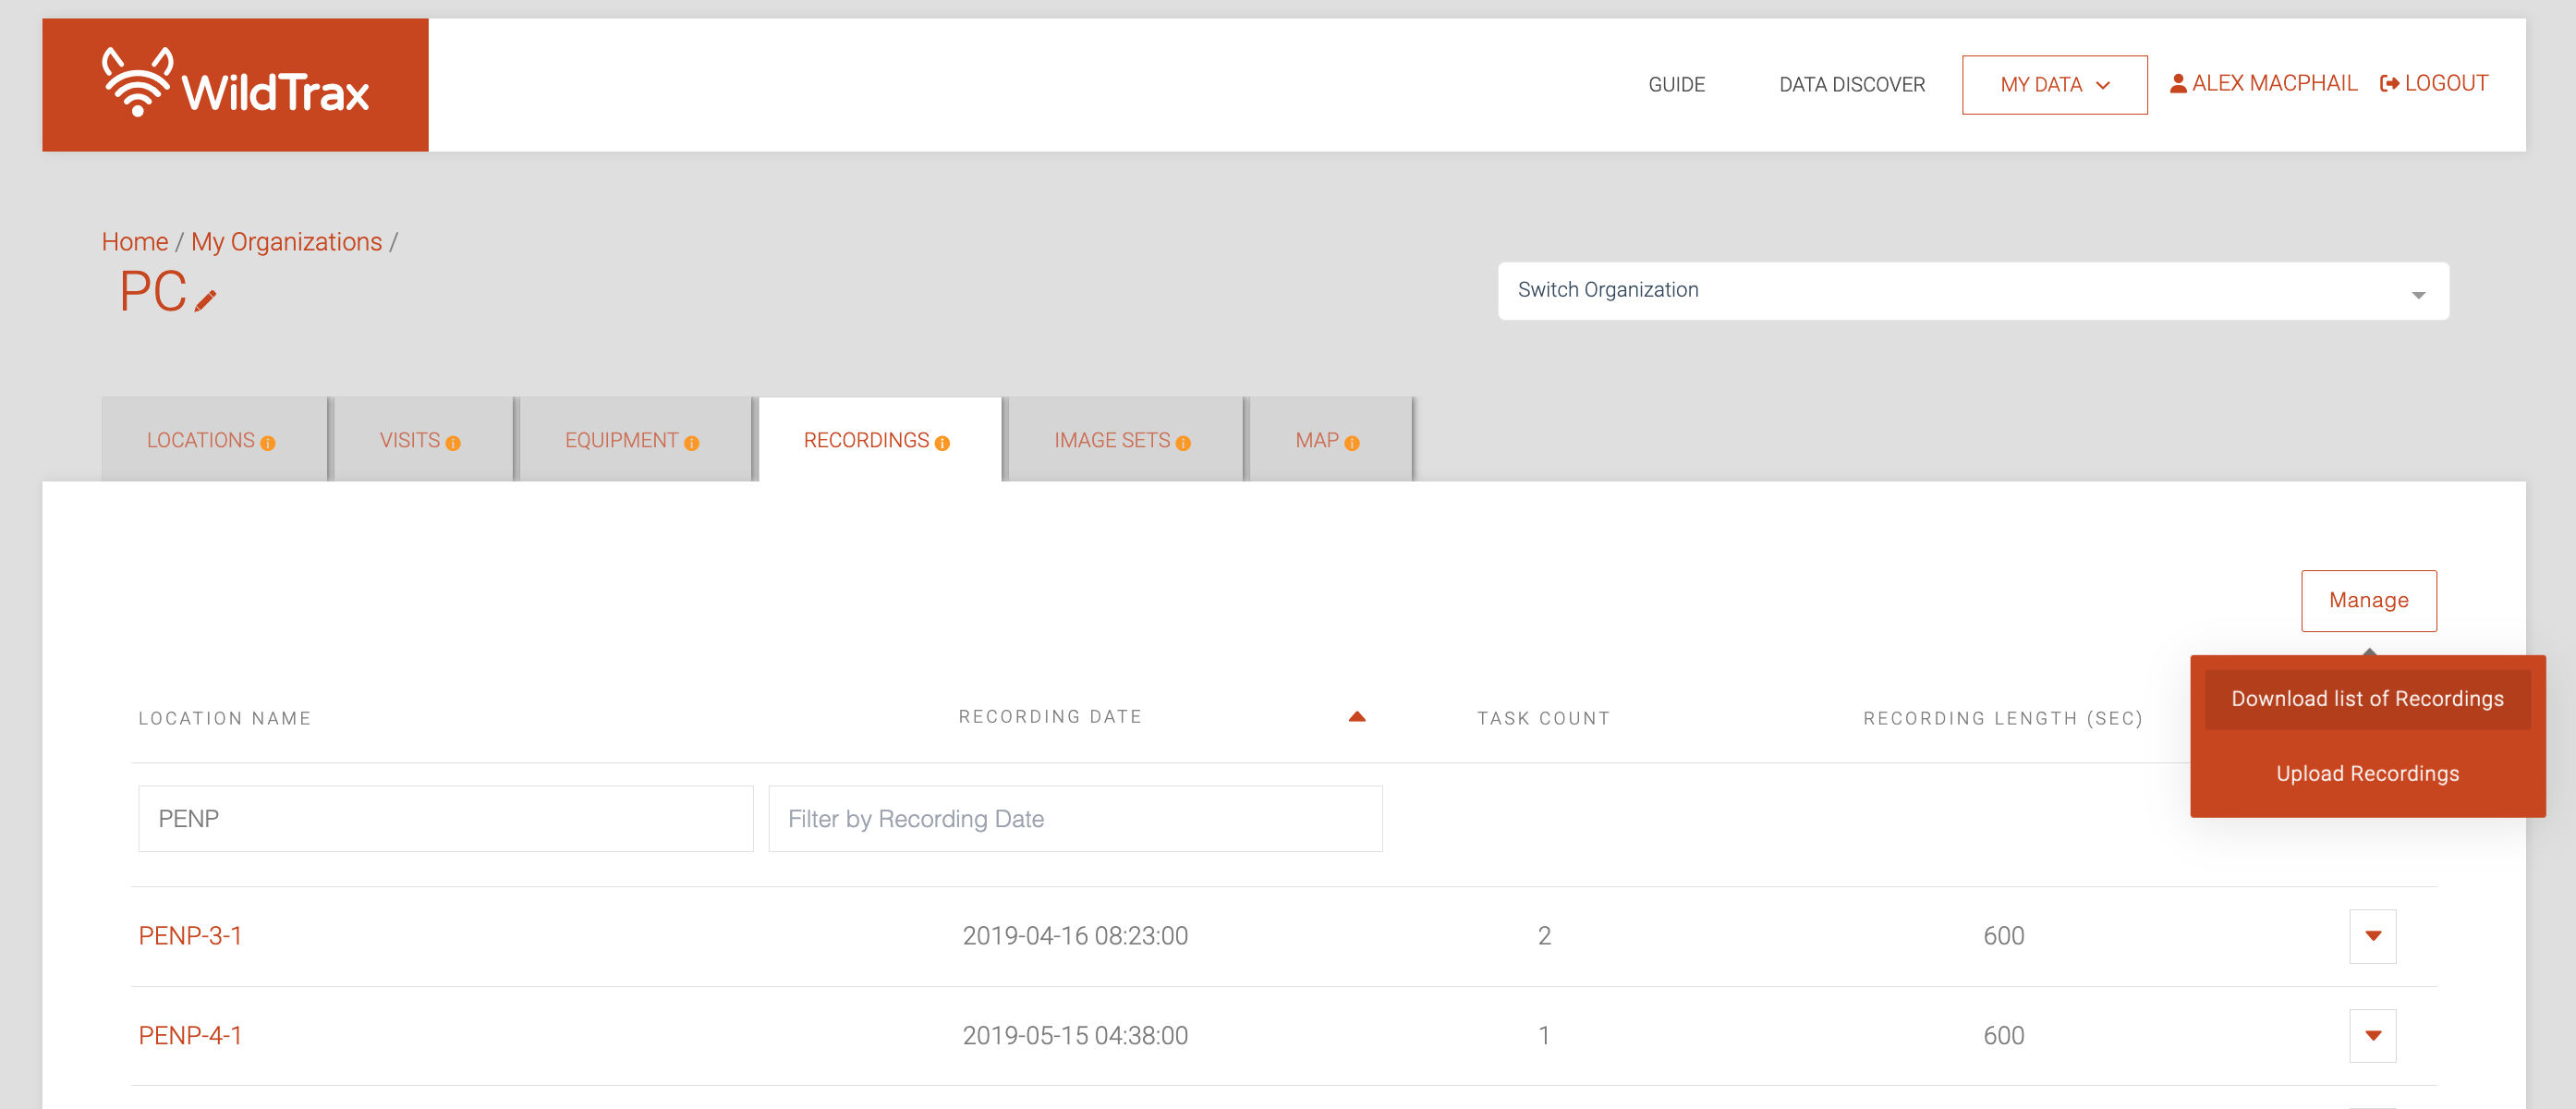
\includegraphics{download-recs.png}

}

\caption{\label{fig-download-recs}Downloading a list of recordings from
WildTrax}

\end{figure}

\begin{figure}

{\centering 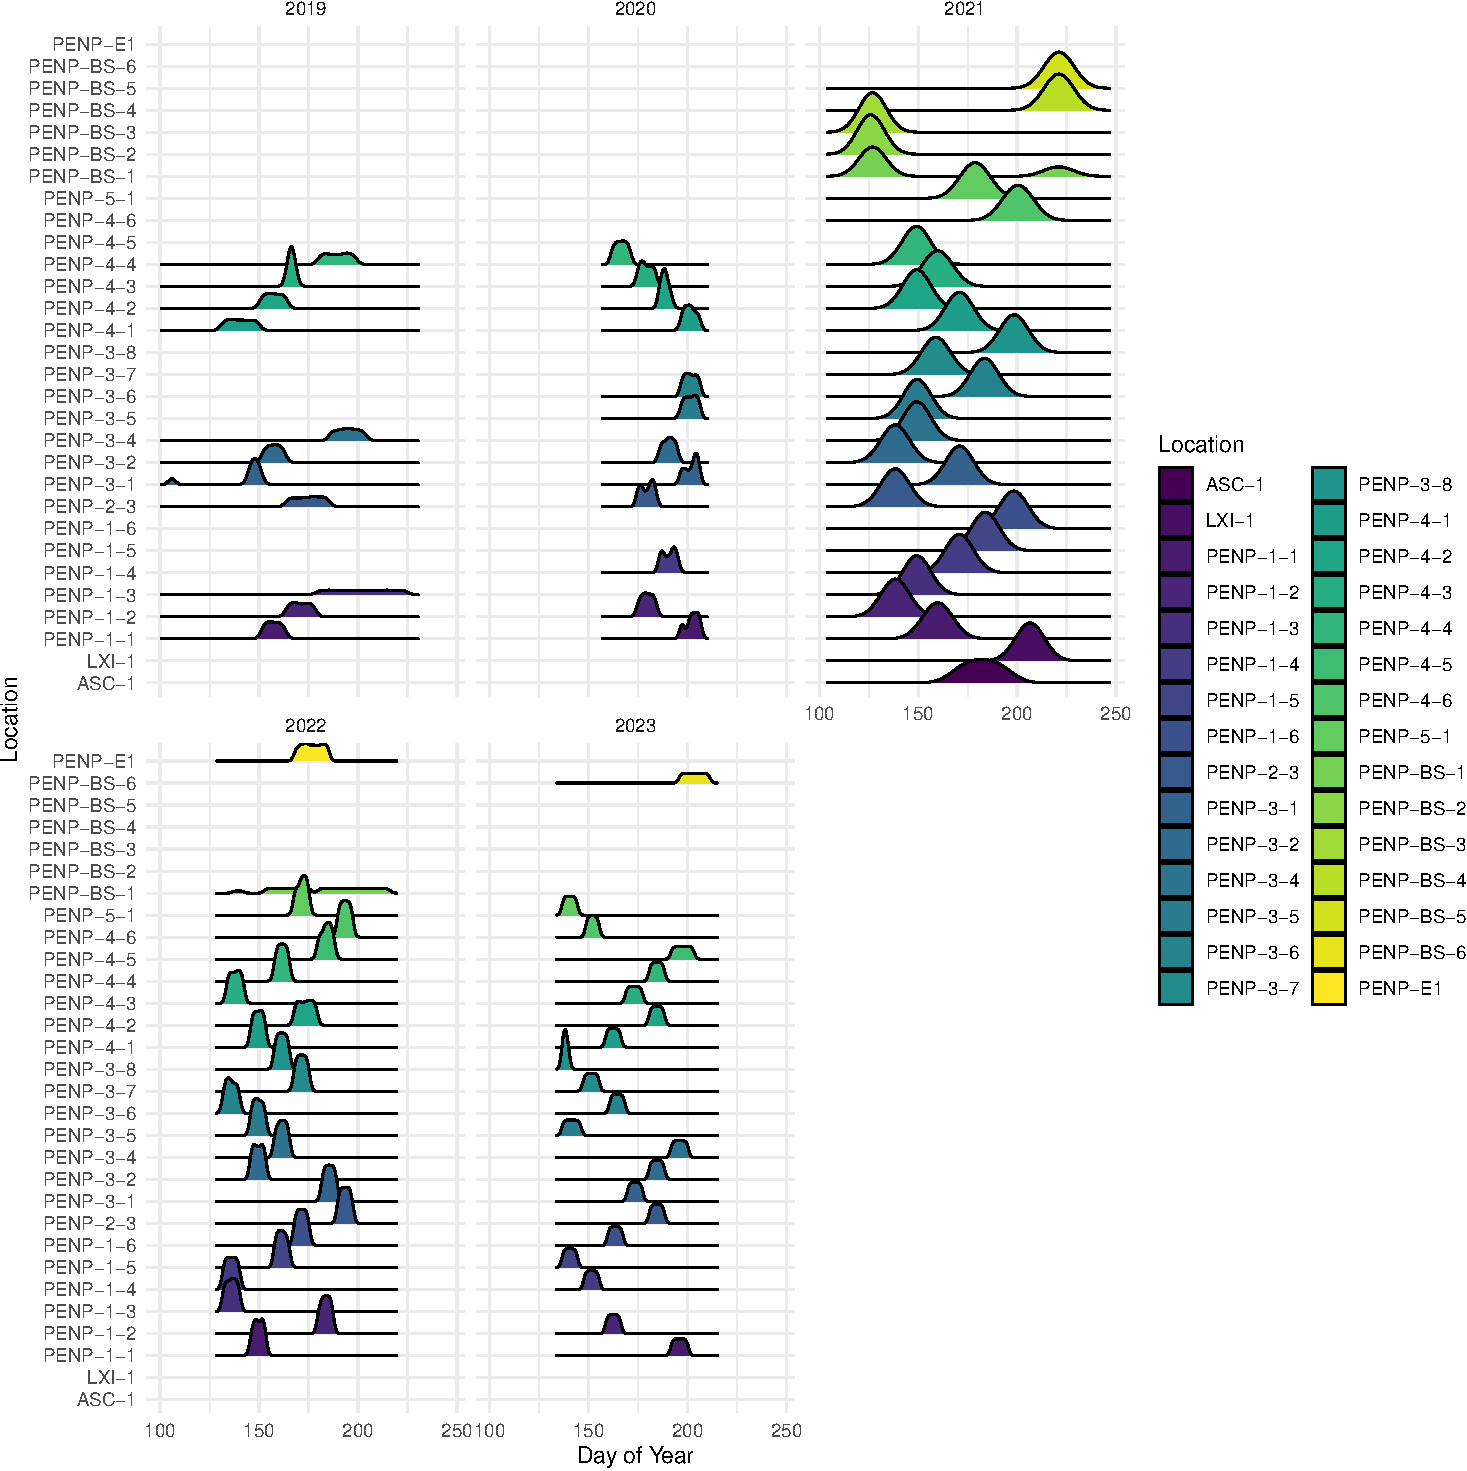
\includegraphics{peinp_files/figure-pdf/fig-recs-collect-1.pdf}

}

\caption{\label{fig-recs-collect}Ridgeplot of recordings collected for
each location over each survey year}

\end{figure}

\hypertarget{community-data-processing}{%
\subsection{Community data processing}\label{community-data-processing}}

The principal goal for data processing was to describe the acoustic
community of species heard at locations while choosing a large enough
subset of recordings for analyses. To ensure balanced replication, for
each location and year surveyed, four randomly selected recordings were
processed for 3-minutes between the hours of 4:00 AM - 7:59 AM ideally
on four separate dates (see Table~\ref{tbl-loc-repl}). Four recordings
will ensure that we have the minimum number of samples for a simple
occupancy analysis. Tags are made in a count-removal framework, only
tagging the time of first detection of each individual heard on the
recordings. In case a species was overly abundant a TMTT (`too many to
tag') flag was used (see Table~\ref{tbl-tmtt}). Amphibian abundance was
estimated at the time of first detection using the
\href{https://www.usgs.gov/centers/eesc/science/north-american-amphibian-monitoring-program}{North
American Amphibian Monitoring Program} with abundance of species being
estimated on the scale of ``calling intensity index'' of 1 - 3. Mammals
such as Red Squirrel, were also noted on the recordings. After the data
are processed in WildTrax, the
\href{https://abbiodiversity.github.io/wildRtrax/}{wildRtrax} package is
use to download the data into a standard format prepared for analysis.
We also verified that all tags that were created were checked by a
second observer to ensure accuracy of detections (see
Table~\ref{tbl-verified}).

\hypertarget{tbl-loc-repl}{}
\begin{table}
\caption{\label{tbl-loc-repl}Example of tasks and unit replication for listening at PENP-1-1 }\tabularnewline

\centering
\begin{tabular}{l|r|l|l|r}
\hline
location & year & task\_duration & typ & n\\
\hline
PENP-1-1 & 2019 & 180s & Dawn & 6\\
\hline
PENP-1-1 & 2019 & 180s & Day & 7\\
\hline
PENP-1-1 & 2020 & 180s & Dawn & 9\\
\hline
PENP-1-1 & 2020 & 180s & Day & 2\\
\hline
PENP-1-1 & 2021 & 180s & Night & 4\\
\hline
PENP-1-1 & 2022 & 180s & Dawn & 4\\
\hline
PENP-1-1 & 2023 & 180s & Dawn & 4\\
\hline
\end{tabular}
\end{table}

\hypertarget{tbl-verified}{}
\begin{table}
\caption{\label{tbl-verified}Proportion of tags verified }\tabularnewline

\centering
\begin{tabular}{l|r|r}
\hline
Tag is verified & Count & Proportion\\
\hline
 & 168 & 1.65\\
\hline
f & 2927 & 28.82\\
\hline
t & 7060 & 69.52\\
\hline
\end{tabular}
\end{table}

\hypertarget{tbl-tmtt}{}
\begin{table}
\caption{\label{tbl-tmtt}TMTT tags }\tabularnewline

\centering
\begin{tabular}{l|l|l|l}
\hline
location & recording\_date\_time & species\_code & individual\_count\\
\hline
PENP-1-1 & 2019-06-01 05:25:00 & AMCR & TMTT\\
\hline
PENP-1-1 & 2019-06-01 05:25:00 & AMRE & TMTT\\
\hline
PENP-1-1 & 2019-06-02 06:24:00 & YEWA & TMTT\\
\hline
PENP-1-1 & 2019-06-02 06:24:00 & AMCR & TMTT\\
\hline
PENP-1-1 & 2019-06-02 06:24:00 & AMRE & TMTT\\
\hline
PENP-1-1 & 2019-06-04 07:23:00 & AMRE & TMTT\\
\hline
\end{tabular}
\end{table}

\hypertarget{visual-scanning}{%
\subsection{Visual scanning}\label{visual-scanning}}

Visual scanning is the concept of visually examining recordings en masse
in order to find the signal in question in audio recordings. It has been
a well-proven method for detecting many different taxa (Cameron et al.
(2020)\marginpar{\begin{footnotesize}\leavevmode\vadjust pre{\protect\hypertarget{ref-vis-scan-amphs}{}}%
Cameron, J., A. Crosby, C. Paszkowski, and E. Bayne. 2020. {``Visual
Spectrogram Scanning Paired with an Observation--Confirmation Occupancy
Model Improves the Efficiency and Accuracy of Bioacoustic Anuran
Data.''} \emph{Canadian Journal of Zoology} 98 (11): 733--42.
\url{https://doi.org/10.1139/cjz-2020-0103}.\vspace{2mm}\par\end{footnotesize}},
(\textbf{arus-vs-cams-wolves?})\marginpar{\begin{footnotesize}arus-vs-cams-wolves\vspace{2mm}\par\end{footnotesize}})
with comparable biological metrics to other traditional methods. Visual
scanning allows a user to use frequency-limited or time-limited
spectrograms and scan lots of them visually much faster than listening
to the audio. These changes are easily made by adjusting project
settings in WildTrax. Visual scanning for Bank Swallow was conducted at
each \texttt{PENP-BS-*} location. A total of 0 recordings. Tags were
made at the time of first detection in each minute interval.

\hypertarget{automated-recognition}{%
\subsection{Automated recognition}\label{automated-recognition}}

Automated recognition is a well-known process to help detect rare and
elusive species, as well as species that may have low detectability in
large data sets. We constructed a recognizer for EAWP and used three
previously constructed Wildlife Acoustics SongScope recognizer for OSFL,
RUBL and CAWA. Hits were uploaded to WildTrax via the
\texttt{wt\_songscope\_tags} function in \texttt{wildRtrax}.

\begin{Shaded}
\begin{Highlighting}[]
\FunctionTok{wt\_songscope\_tags}\NormalTok{()}
\end{Highlighting}
\end{Shaded}

\begin{center}\rule{0.5\linewidth}{0.5pt}\end{center}

\hypertarget{results}{%
\section{Results}\label{results}}

\hypertarget{avian-species}{%
\subsection{Avian species}\label{avian-species}}

\hypertarget{species-richness}{%
\subsubsection{Species richness}\label{species-richness}}

A total of 100 species were found across the five years.
Figure~\ref{fig-spp-rich-locs} describes the relationship of species
richness across each location and survey year with
Figure~\ref{fig-spp-rich-annual} showing the relationship between
species richness and survey effort.

\begin{figure}

{\centering 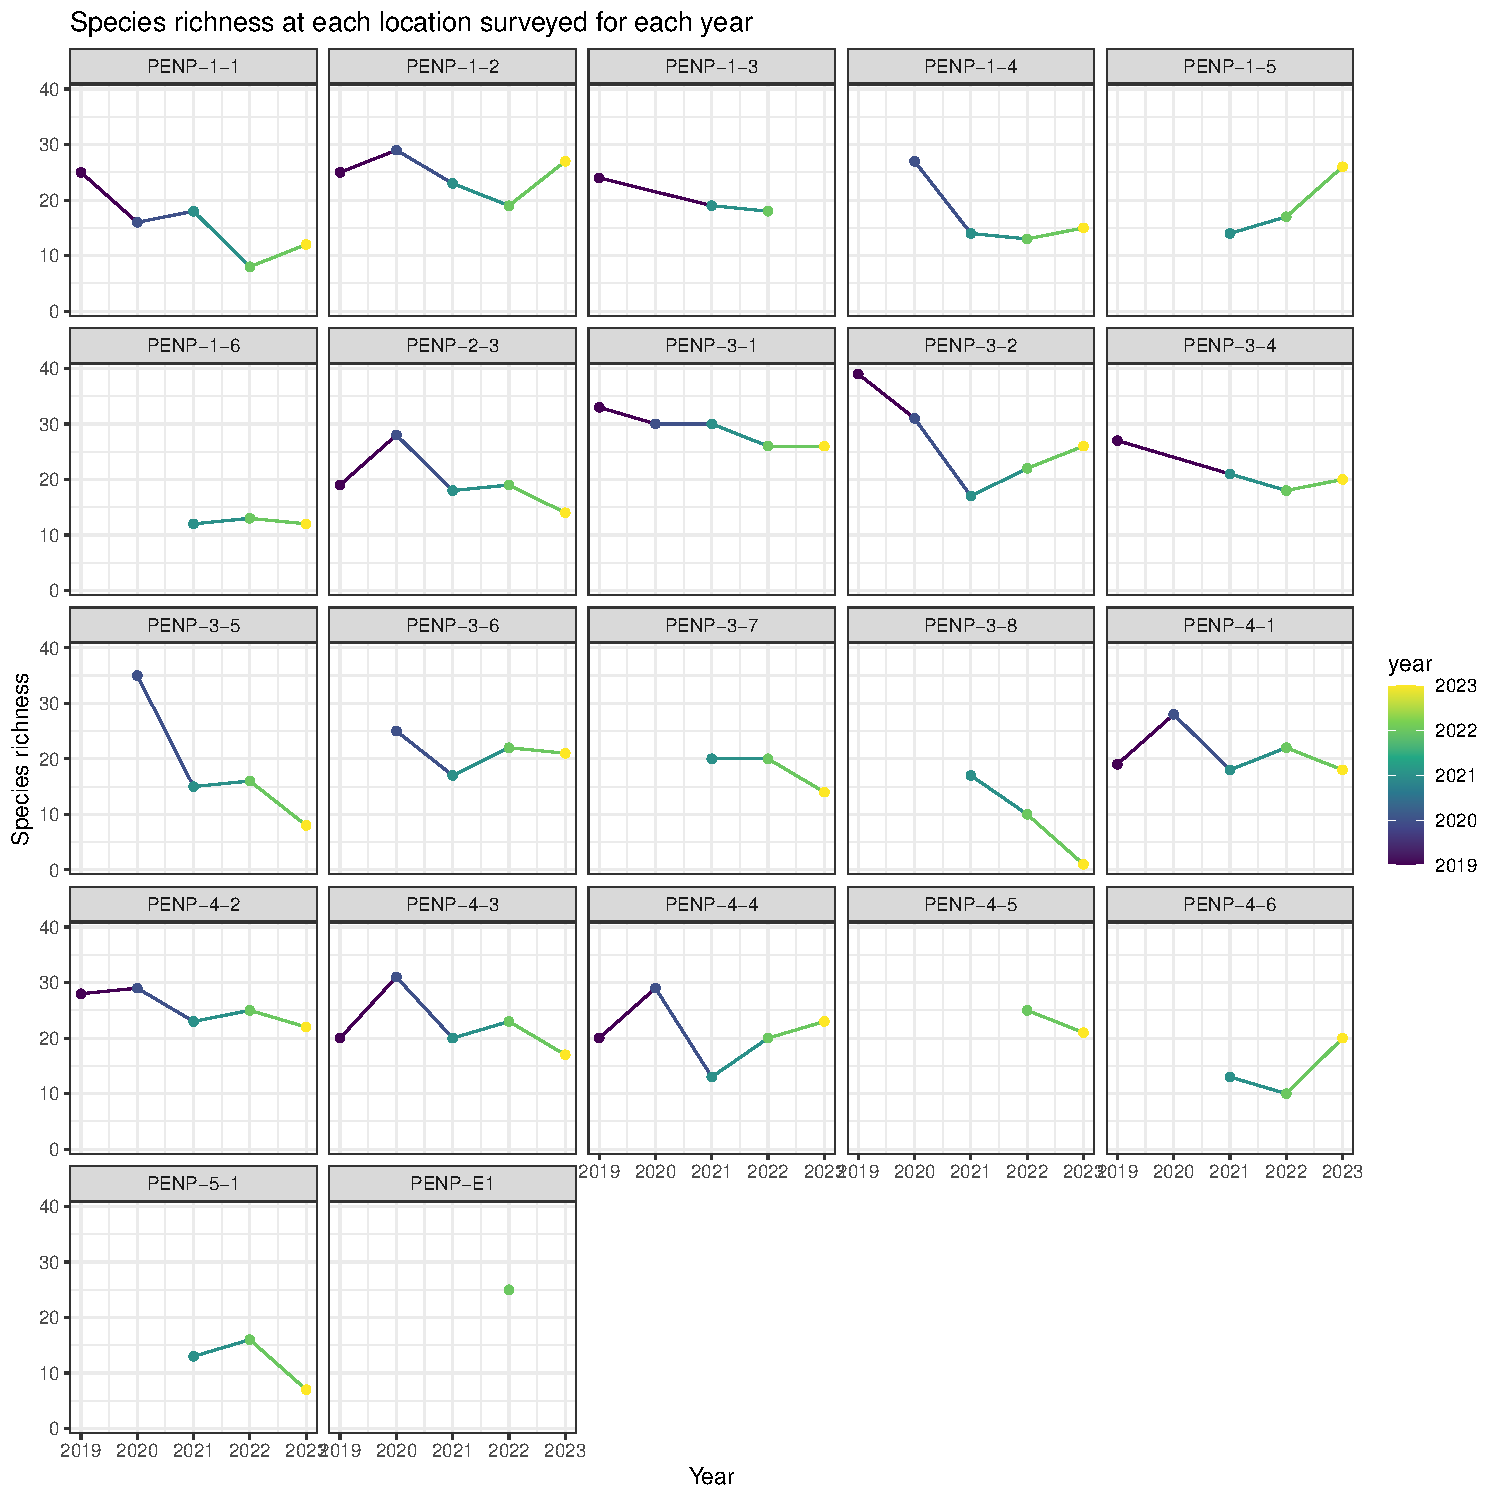
\includegraphics{peinp_files/figure-pdf/fig-spp-rich-locs-1.pdf}

}

\caption{\label{fig-spp-rich-locs}Species richness at forest monitoring
locations across years}

\end{figure}

\begin{figure}

{\centering 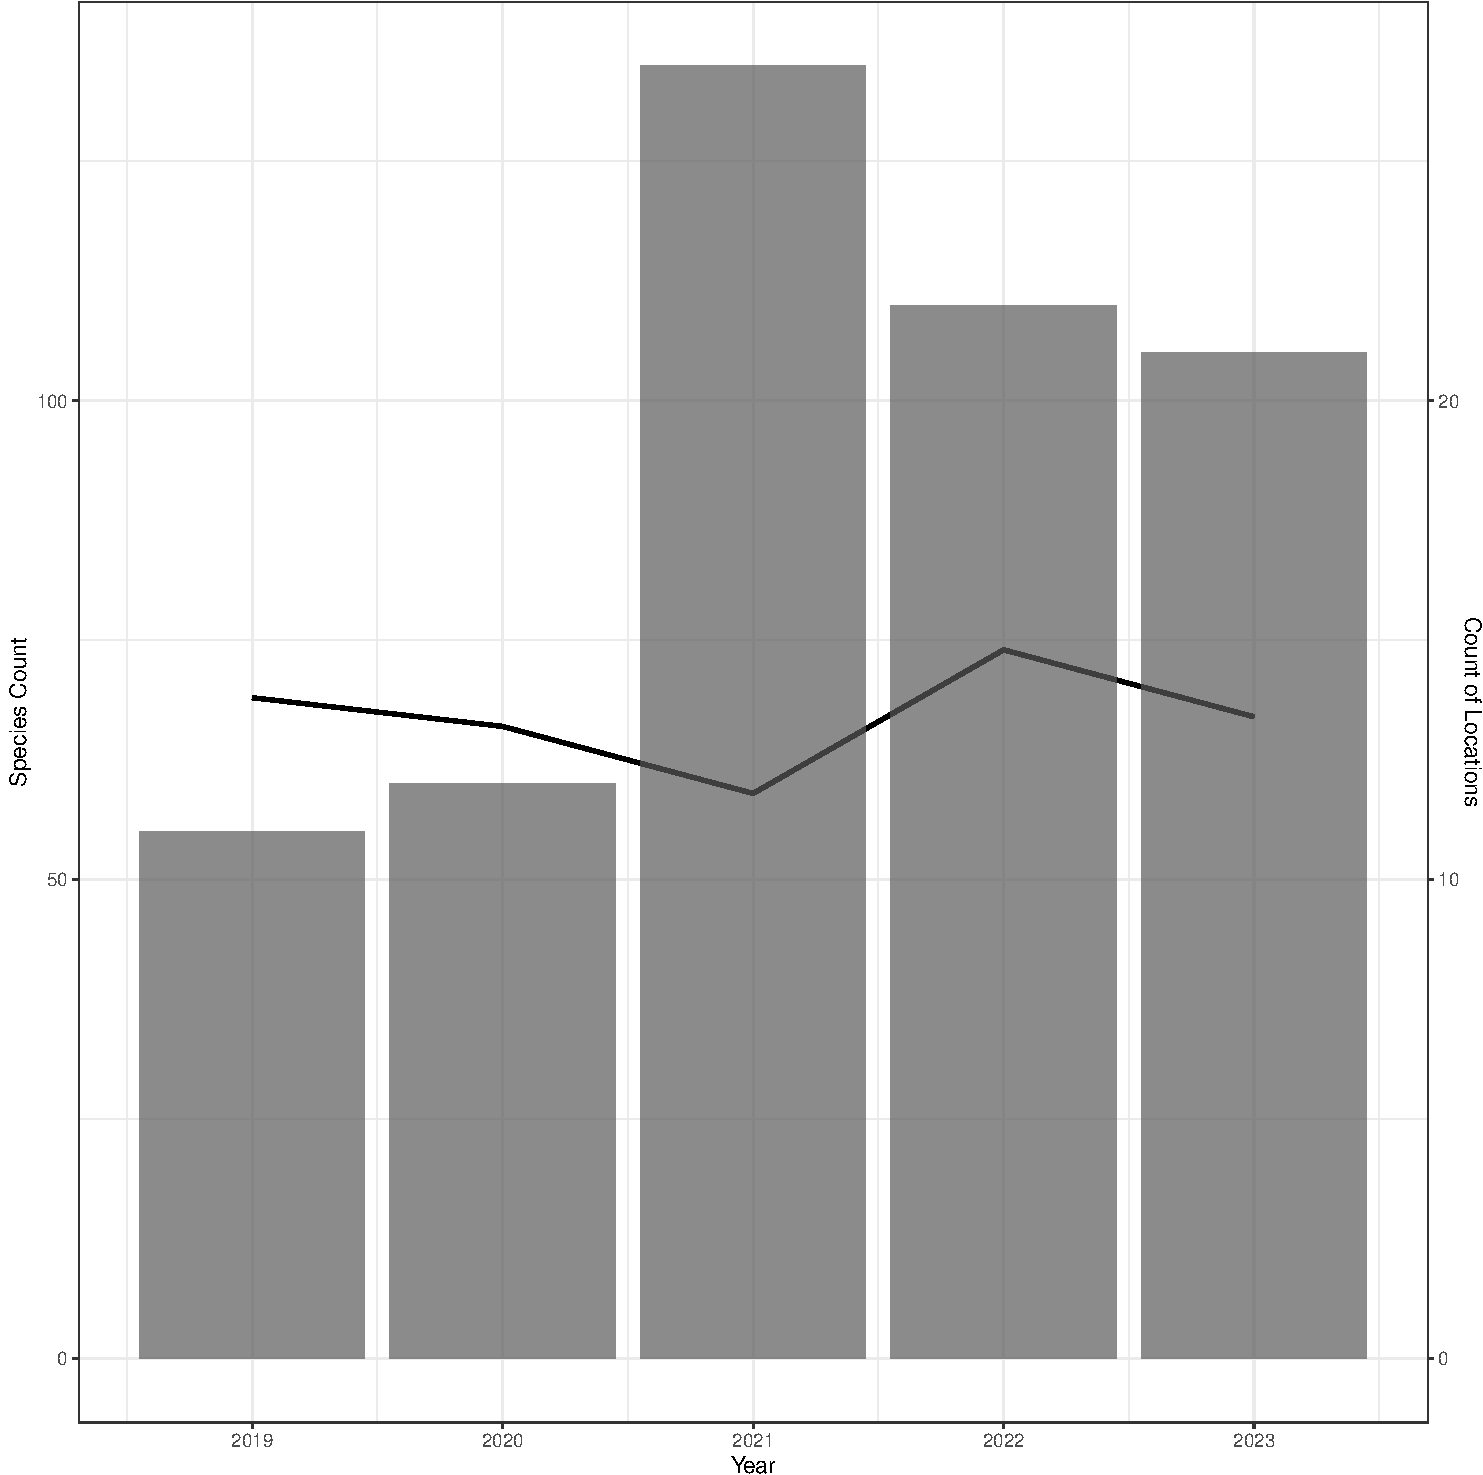
\includegraphics{peinp_files/figure-pdf/fig-spp-rich-annual-1.pdf}

}

\caption{\label{fig-spp-rich-annual}Species richness at forest
monitoring locations across years considering sampling effort}

\end{figure}

\begin{figure}

{\centering 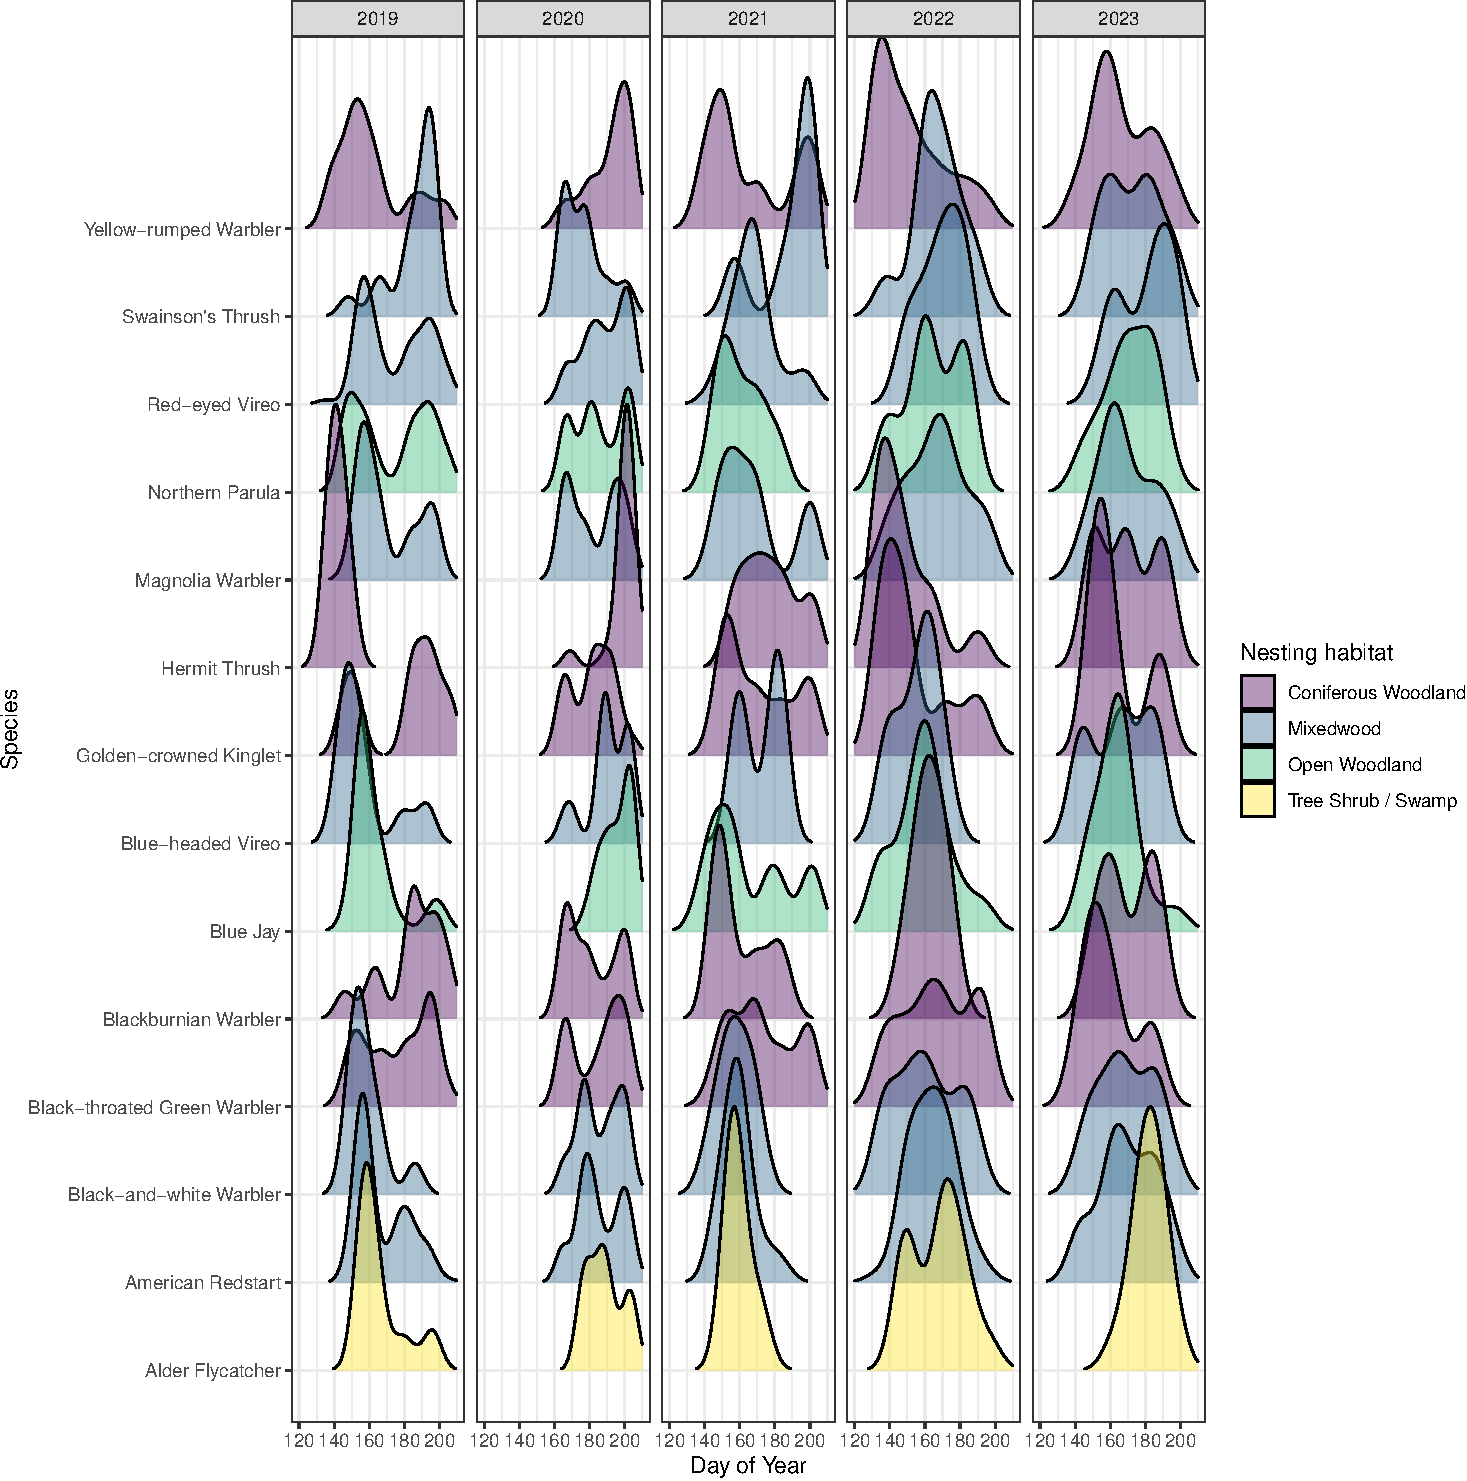
\includegraphics{peinp_files/figure-pdf/fig-spp-activity-1.pdf}

}

\caption{\label{fig-spp-activity}Seasonal detection activity of most
commonly detected forest species}

\end{figure}

A quick test to show proximity to ocean is the major effect of noise and
species richness on audio data so that we can use that site covariate in
the occupany models.

\hypertarget{species-diversity}{%
\subsubsection{Species diversity}\label{species-diversity}}

\begin{Shaded}
\begin{Highlighting}[]
\NormalTok{raw\_dog }\OtherTok{\textless{}{-}}\NormalTok{ pei\_main }\SpecialCharTok{|\textgreater{}} 
  \FunctionTok{as\_tibble}\NormalTok{() }\SpecialCharTok{|\textgreater{}}
  \FunctionTok{wt\_tidy\_species}\NormalTok{(}\AttributeTok{remove =} \FunctionTok{c}\NormalTok{(}\StringTok{"mammal"}\NormalTok{,}\StringTok{"amphibian"}\NormalTok{,}\StringTok{"abiotic"}\NormalTok{,}\StringTok{"insect"}\NormalTok{,}\StringTok{"unknown"}\NormalTok{), }\AttributeTok{zerofill =}\NormalTok{ T) }\SpecialCharTok{|\textgreater{}}
  \FunctionTok{filter}\NormalTok{(}\SpecialCharTok{!}\FunctionTok{grepl}\NormalTok{(}\StringTok{\textquotesingle{}BS|ASC|LXI\textquotesingle{}}\NormalTok{,location)) }\SpecialCharTok{|\textgreater{}}
  \FunctionTok{wt\_replace\_tmtt}\NormalTok{() }\SpecialCharTok{|\textgreater{}}
  \FunctionTok{select}\NormalTok{(location, recording\_date\_time, species\_code, species\_common\_name, individual\_order, individual\_count) }\SpecialCharTok{|\textgreater{}}
  \FunctionTok{distinct}\NormalTok{() }\SpecialCharTok{|\textgreater{}}
  \FunctionTok{group\_by}\NormalTok{(location, recording\_date\_time, species\_code, species\_common\_name) }\SpecialCharTok{|\textgreater{}}
  \FunctionTok{summarise}\NormalTok{(}\AttributeTok{count =} \FunctionTok{max}\NormalTok{(individual\_order)) }\SpecialCharTok{|\textgreater{}}
  \FunctionTok{ungroup}\NormalTok{() }\SpecialCharTok{|\textgreater{}}
  \FunctionTok{pivot\_wider}\NormalTok{(}\AttributeTok{names\_from =}\NormalTok{ species\_code, }\AttributeTok{values\_from =}\NormalTok{ count, }\AttributeTok{values\_fill =} \DecValTok{0}\NormalTok{) }\SpecialCharTok{|\textgreater{}}
  \FunctionTok{as.data.frame}\NormalTok{()}
\end{Highlighting}
\end{Shaded}

\begin{verbatim}

Downloading: 8.2 kB     
Downloading: 8.2 kB     
Downloading: 8.2 kB     
Downloading: 8.2 kB     
Downloading: 8.2 kB     
Downloading: 8.2 kB     
Downloading: 8.2 kB     
Downloading: 8.2 kB     
Downloading: 16 kB     
Downloading: 16 kB     
Downloading: 16 kB     
Downloading: 16 kB     
Downloading: 16 kB     
Downloading: 16 kB     
Downloading: 25 kB     
Downloading: 25 kB     
Downloading: 25 kB     
Downloading: 25 kB     
Downloading: 25 kB     
Downloading: 25 kB     
Downloading: 33 kB     
Downloading: 33 kB     
Downloading: 33 kB     
Downloading: 33 kB     
Downloading: 33 kB     
Downloading: 33 kB     
Downloading: 33 kB     
Downloading: 33 kB     
Downloading: 41 kB     
Downloading: 41 kB     
Downloading: 41 kB     
Downloading: 41 kB     
Downloading: 41 kB     
Downloading: 41 kB     
Downloading: 49 kB     
Downloading: 49 kB     
Downloading: 49 kB     
Downloading: 49 kB     
Downloading: 49 kB     
Downloading: 49 kB     
Downloading: 57 kB     
Downloading: 57 kB     
Downloading: 57 kB     
Downloading: 57 kB     
Downloading: 57 kB     
Downloading: 57 kB     
Downloading: 65 kB     
Downloading: 65 kB     
Downloading: 65 kB     
Downloading: 65 kB     
Downloading: 65 kB     
Downloading: 65 kB     
Downloading: 74 kB     
Downloading: 74 kB     
Downloading: 74 kB     
Downloading: 74 kB     
Downloading: 74 kB     
Downloading: 74 kB     
Downloading: 82 kB     
Downloading: 82 kB     
Downloading: 82 kB     
Downloading: 82 kB     
Downloading: 82 kB     
Downloading: 82 kB     
Downloading: 90 kB     
Downloading: 90 kB     
Downloading: 90 kB     
Downloading: 90 kB     
Downloading: 90 kB     
Downloading: 90 kB     
Downloading: 90 kB     
Downloading: 90 kB     
Downloading: 98 kB     
Downloading: 98 kB     
Downloading: 98 kB     
Downloading: 98 kB     
Downloading: 98 kB     
Downloading: 98 kB     
Downloading: 110 kB     
Downloading: 110 kB     
Downloading: 110 kB     
Downloading: 110 kB     
Downloading: 110 kB     
Downloading: 110 kB     
Downloading: 110 kB     
Downloading: 110 kB     
Downloading: 110 kB     
Downloading: 110 kB     
Downloading: 110 kB     
Downloading: 110 kB     
Downloading: 120 kB     
Downloading: 120 kB     
Downloading: 120 kB     
Downloading: 120 kB     
Downloading: 120 kB     
Downloading: 120 kB     
Downloading: 130 kB     
Downloading: 130 kB     
Downloading: 130 kB     
Downloading: 130 kB     
Downloading: 130 kB     
Downloading: 130 kB     
Downloading: 140 kB     
Downloading: 140 kB     
Downloading: 140 kB     
Downloading: 140 kB     
Downloading: 140 kB     
Downloading: 140 kB     
Downloading: 150 kB     
Downloading: 150 kB     
Downloading: 150 kB     
Downloading: 150 kB     
Downloading: 150 kB     
Downloading: 150 kB     
Downloading: 160 kB     
Downloading: 160 kB     
Downloading: 160 kB     
Downloading: 160 kB     
Downloading: 160 kB     
Downloading: 160 kB     
Downloading: 160 kB     
Downloading: 160 kB     
Downloading: 160 kB     
Downloading: 160 kB     
Downloading: 160 kB     
Downloading: 160 kB     
Downloading: 170 kB     
Downloading: 170 kB     
Downloading: 170 kB     
Downloading: 170 kB     
Downloading: 170 kB     
Downloading: 170 kB     
Downloading: 180 kB     
Downloading: 180 kB     
Downloading: 180 kB     
Downloading: 180 kB     
Downloading: 180 kB     
Downloading: 180 kB     
Downloading: 190 kB     
Downloading: 190 kB     
Downloading: 190 kB     
Downloading: 190 kB     
Downloading: 190 kB     
Downloading: 190 kB     
Downloading: 200 kB     
Downloading: 200 kB     
Downloading: 200 kB     
Downloading: 200 kB     
Downloading: 200 kB     
Downloading: 200 kB     
Downloading: 200 kB     
Downloading: 200 kB     
Downloading: 200 kB     
Downloading: 200 kB     
Downloading: 200 kB     
Downloading: 200 kB     
Downloading: 200 kB     
Downloading: 200 kB     
Downloading: 210 kB     
Downloading: 210 kB     
Downloading: 210 kB     
Downloading: 210 kB     
Downloading: 210 kB     
Downloading: 210 kB     
Downloading: 220 kB     
Downloading: 220 kB     
Downloading: 220 kB     
Downloading: 220 kB     
Downloading: 220 kB     
Downloading: 220 kB     
Downloading: 230 kB     
Downloading: 230 kB     
Downloading: 230 kB     
Downloading: 230 kB     
Downloading: 230 kB     
Downloading: 230 kB     
Downloading: 240 kB     
Downloading: 240 kB     
Downloading: 240 kB     
Downloading: 240 kB     
Downloading: 240 kB     
Downloading: 240 kB     
Downloading: 250 kB     
Downloading: 250 kB     
Downloading: 250 kB     
Downloading: 250 kB     
Downloading: 250 kB     
Downloading: 250 kB     
Downloading: 250 kB     
Downloading: 250 kB     
Downloading: 250 kB     
Downloading: 250 kB     
Downloading: 250 kB     
Downloading: 250 kB     
Downloading: 260 kB     
Downloading: 260 kB     
Downloading: 260 kB     
Downloading: 260 kB     
Downloading: 260 kB     
Downloading: 260 kB     
Downloading: 270 kB     
Downloading: 270 kB     
Downloading: 270 kB     
Downloading: 270 kB     
Downloading: 270 kB     
Downloading: 270 kB     
Downloading: 280 kB     
Downloading: 280 kB     
Downloading: 280 kB     
Downloading: 280 kB     
Downloading: 280 kB     
Downloading: 280 kB     
Downloading: 290 kB     
Downloading: 290 kB     
Downloading: 290 kB     
Downloading: 290 kB     
Downloading: 290 kB     
Downloading: 290 kB     
Downloading: 290 kB     
Downloading: 290 kB     
Downloading: 290 kB     
Downloading: 290 kB     
Downloading: 290 kB     
Downloading: 290 kB     
Downloading: 300 kB     
Downloading: 300 kB     
Downloading: 300 kB     
Downloading: 300 kB     
Downloading: 300 kB     
Downloading: 300 kB     
Downloading: 310 kB     
Downloading: 310 kB     
Downloading: 310 kB     
Downloading: 310 kB     
Downloading: 310 kB     
Downloading: 310 kB     
Downloading: 320 kB     
Downloading: 320 kB     
Downloading: 320 kB     
Downloading: 320 kB     
Downloading: 320 kB     
Downloading: 320 kB     
Downloading: 330 kB     
Downloading: 330 kB     
Downloading: 330 kB     
Downloading: 330 kB     
Downloading: 330 kB     
Downloading: 330 kB     
Downloading: 340 kB     
Downloading: 340 kB     
Downloading: 340 kB     
Downloading: 340 kB     
Downloading: 340 kB     
Downloading: 340 kB     
Downloading: 340 kB     
Downloading: 340 kB     
Downloading: 340 kB     
Downloading: 340 kB     
Downloading: 340 kB     
Downloading: 340 kB     
Downloading: 350 kB     
Downloading: 350 kB     
Downloading: 350 kB     
Downloading: 350 kB     
Downloading: 350 kB     
Downloading: 350 kB     
Downloading: 360 kB     
Downloading: 360 kB     
Downloading: 360 kB     
Downloading: 360 kB     
Downloading: 360 kB     
Downloading: 360 kB     
Downloading: 370 kB     
Downloading: 370 kB     
Downloading: 370 kB     
Downloading: 370 kB     
Downloading: 370 kB     
Downloading: 370 kB     
Downloading: 380 kB     
Downloading: 380 kB     
Downloading: 380 kB     
Downloading: 380 kB     
Downloading: 380 kB     
Downloading: 380 kB     
Downloading: 380 kB     
Downloading: 380 kB     
Downloading: 380 kB     
Downloading: 380 kB     
Downloading: 380 kB     
Downloading: 380 kB     
Downloading: 390 kB     
Downloading: 390 kB     
Downloading: 390 kB     
Downloading: 390 kB     
Downloading: 390 kB     
Downloading: 390 kB     
Downloading: 400 kB     
Downloading: 400 kB     
Downloading: 400 kB     
Downloading: 400 kB     
Downloading: 400 kB     
Downloading: 400 kB     
Downloading: 410 kB     
Downloading: 410 kB     
Downloading: 410 kB     
Downloading: 410 kB     
Downloading: 410 kB     
Downloading: 410 kB     
Downloading: 410 kB     
Downloading: 410 kB     
Downloading: 420 kB     
Downloading: 420 kB     
Downloading: 420 kB     
Downloading: 420 kB     
Downloading: 420 kB     
Downloading: 420 kB     
Downloading: 430 kB     
Downloading: 430 kB     
Downloading: 430 kB     
Downloading: 430 kB     
Downloading: 430 kB     
Downloading: 430 kB     
Downloading: 430 kB     
Downloading: 430 kB     
Downloading: 430 kB     
Downloading: 430 kB     
Downloading: 430 kB     
Downloading: 430 kB     
Downloading: 440 kB     
Downloading: 440 kB     
Downloading: 440 kB     
Downloading: 440 kB     
Downloading: 440 kB     
Downloading: 440 kB     
Downloading: 450 kB     
Downloading: 450 kB     
Downloading: 450 kB     
Downloading: 450 kB     
Downloading: 450 kB     
Downloading: 450 kB     
Downloading: 460 kB     
Downloading: 460 kB     
Downloading: 460 kB     
Downloading: 460 kB     
Downloading: 460 kB     
Downloading: 460 kB     
Downloading: 470 kB     
Downloading: 470 kB     
Downloading: 470 kB     
Downloading: 470 kB     
Downloading: 470 kB     
Downloading: 470 kB     
Downloading: 470 kB     
Downloading: 470 kB     
Downloading: 470 kB     
Downloading: 470 kB     
Downloading: 470 kB     
Downloading: 470 kB     
Downloading: 480 kB     
Downloading: 480 kB     
Downloading: 480 kB     
Downloading: 480 kB     
Downloading: 480 kB     
Downloading: 480 kB     
Downloading: 490 kB     
Downloading: 490 kB     
Downloading: 490 kB     
Downloading: 490 kB     
Downloading: 490 kB     
Downloading: 490 kB     
Downloading: 500 kB     
Downloading: 500 kB     
Downloading: 500 kB     
Downloading: 500 kB     
Downloading: 500 kB     
Downloading: 500 kB     
Downloading: 510 kB     
Downloading: 510 kB     
Downloading: 510 kB     
Downloading: 510 kB     
Downloading: 510 kB     
Downloading: 510 kB     
Downloading: 520 kB     
Downloading: 520 kB     
Downloading: 520 kB     
Downloading: 520 kB     
Downloading: 520 kB     
Downloading: 520 kB     
Downloading: 520 kB     
Downloading: 520 kB     
Downloading: 520 kB     
Downloading: 520 kB     
Downloading: 520 kB     
Downloading: 520 kB     
Downloading: 530 kB     
Downloading: 530 kB     
Downloading: 530 kB     
Downloading: 530 kB     
Downloading: 530 kB     
Downloading: 530 kB     
Downloading: 540 kB     
Downloading: 540 kB     
Downloading: 540 kB     
Downloading: 540 kB     
Downloading: 540 kB     
Downloading: 540 kB     
Downloading: 550 kB     
Downloading: 550 kB     
Downloading: 550 kB     
Downloading: 550 kB     
Downloading: 550 kB     
Downloading: 550 kB     
Downloading: 560 kB     
Downloading: 560 kB     
Downloading: 560 kB     
Downloading: 560 kB     
Downloading: 560 kB     
Downloading: 560 kB     
Downloading: 560 kB     
Downloading: 560 kB     
Downloading: 560 kB     
Downloading: 560 kB     
Downloading: 560 kB     
Downloading: 560 kB     
Downloading: 570 kB     
Downloading: 570 kB     
Downloading: 570 kB     
Downloading: 570 kB     
Downloading: 570 kB     
Downloading: 570 kB     
Downloading: 580 kB     
Downloading: 580 kB     
Downloading: 580 kB     
Downloading: 580 kB     
Downloading: 580 kB     
Downloading: 580 kB     
Downloading: 590 kB     
Downloading: 590 kB     
Downloading: 590 kB     
Downloading: 590 kB     
Downloading: 590 kB     
Downloading: 590 kB     
Downloading: 600 kB     
Downloading: 600 kB     
Downloading: 600 kB     
Downloading: 600 kB     
Downloading: 600 kB     
Downloading: 600 kB     
Downloading: 610 kB     
Downloading: 610 kB     
Downloading: 610 kB     
Downloading: 610 kB     
Downloading: 610 kB     
Downloading: 610 kB     
Downloading: 610 kB     
Downloading: 610 kB     
Downloading: 610 kB     
Downloading: 610 kB     
Downloading: 610 kB     
Downloading: 610 kB     
Downloading: 620 kB     
Downloading: 620 kB     
Downloading: 620 kB     
Downloading: 620 kB     
Downloading: 620 kB     
Downloading: 620 kB     
Downloading: 630 kB     
Downloading: 630 kB     
Downloading: 630 kB     
Downloading: 630 kB     
Downloading: 630 kB     
Downloading: 630 kB     
Downloading: 630 kB     
Downloading: 630 kB     
\end{verbatim}

\begin{verbatim}
Successfully downloaded the species table!
\end{verbatim}

\begin{verbatim}
`summarise()` has grouped output by 'location', 'recording_date_time',
'species_code'. You can override using the `.groups` argument.
\end{verbatim}

\begin{Shaded}
\begin{Highlighting}[]
\CommentTok{\#betadiver(raw\_dog[,4:103])}
\CommentTok{\#diversity(raw\_dog[,4:103], index="shannon")}
\end{Highlighting}
\end{Shaded}

\hypertarget{species-occupancy}{%
\subsubsection{Species occupancy}\label{species-occupancy}}

For testing species occupancy, we selected locations with a minimum of
four dawn visits across five years, focusing on forest obligate species
for ecological relevance (see \textbf{?@tbl-bird-guilds}). Utilizing a
single-season single-species occupancy model (see
\textbf{?@fig-spp-occ}) from Mackenzie et al.~2003. Site-specific
covariates included the distance to the ocean edge and the proportion of
forested area surrounding the ARU. Observation covariates incorporated
day of the year, hour, observer details, and a quadratic term for both
year and hour. Despite variations in methodology between 2019 (1SPM) and
subsequent years (2020 - 2023), we maintained consistency by exclusively
utilizing the time to the first detection of individuals from the 1SPM
recordings. Model predictions were then generated, and the best model
was selected based on the Aikaike Information Criterion (AIC).

\hypertarget{species-at-risk}{%
\subsubsection{Species-at-risk}\label{species-at-risk}}

\hypertarget{visual-scanning-1}{%
\subsection{Visual scanning}\label{visual-scanning-1}}

\begin{center}\rule{0.5\linewidth}{0.5pt}\end{center}

\hypertarget{amphibians}{%
\subsection{Amphibians}\label{amphibians}}

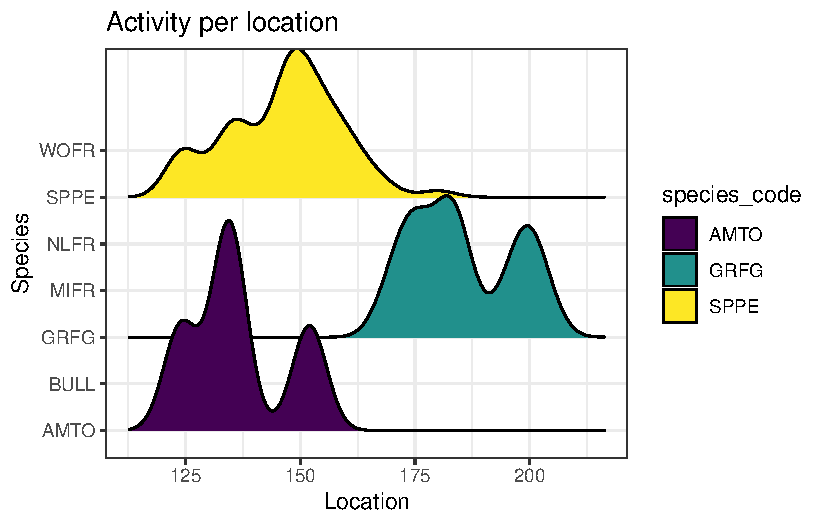
\includegraphics{peinp_files/figure-pdf/unnamed-chunk-22-1.pdf}

\begin{center}\rule{0.5\linewidth}{0.5pt}\end{center}

\hypertarget{discussion}{%
\section{Discussion}\label{discussion}}

\begin{center}\rule{0.5\linewidth}{0.5pt}\end{center}

\hypertarget{references}{%
\subsubsection{References}\label{references}}

\begin{center}\rule{0.5\linewidth}{0.5pt}\end{center}




\end{document}
